\chapter{Hardware and Software Activities Undertaken}
\label{chap:Hardware}

The Hadron Outer (HO) calorimeter of the CMS detector has been installed to measure the energy which is not contained by the barrel calorimeters. The HO improves the energy resolution of highly energetic hadrons and hence provides a better jet energy reconstruction as well as missing transverse energy resolution. HO is situated in the barrel return yokes (YB) in front of the first layer of muon chambers. The YBs consist of 5 rings of iron: YB0, YB$\pm$1 and YB$\pm$2. Rings R0, R$\pm$1 and R$\pm$2 of the HO system are located in YB0, YB$\pm$1 and YB$\pm$2 respectively. In the original design of HO, the signals of the detector were read out by hybrid photo-diodes (HPDs) by converting the wavelength shifted scintillator light into electrical charges. The electronics readout system of the HO is built using the 18-channel readout modules (RMs). The RMs combine the photo-sensors, amplifiers and analogue to digital converters (ADC) and are housed in crates (RBX). The newly developed SiPM system consists of three circuit boards : a mounting Board (MB) holding the SiPMs, a bias board generating the SiPM operation voltage and the a control board connecting the SiPMs electrically to the HCAL readout electronics and monitors the operation of the individual SiPMs. The array of 18 SiPMs is mounted on one side of the MB, as shown in Fig.~\ref{fig:sipm}. The geometrical constraints required a total of 132 RMs to read all channels. The HPDs were chosen as photo-sensors due to its high gain and magnetic field tolerance. But in Run I conditions of the CMS, HPDs proved to be less optimal because of the discharge caused by the fringe field of the CMS magnet, low gain and photo detection efficiency, and ageing effects. Due to these inefficiencies, the HPDs needed to be replaced with multi-pixel Geiger-mode avalanche photo-diodes also known as silicon photo-multipliers (SiPMs). The SiPMs are preferred because of the low operating volatge, relatively high gain, magnetic field insensitivity and high photon-detection efficiency. This replacement was carried out during the first LHC long shutdown (LS1) in 2013-2014 \cite{Lutz:2012yoa}, where the LHC was upgraded to higher luminosity (5 $\times$ 10$^{34} {\rm cm}^2 {\rm s}^{-1}$) and center-of-mass energy of proton-proton collisions was increased from 4 TeV to 6.5 TeV per beam. During this up-gradation, the replacement of HPDs took place in two steps : first the existing RMs with HPDs were taken out from the detector and then were rebuild with SiPMs. After verifying the working of the RMs, they were re-installed in the CMS detector. In collaboration with HO group of the CMS, we participated in the re-installation of the RMs with SiPMs in place of HPDs specially in the sectors YB\plusn 1 and YB\plusn 2 of HCAL during the visit to CERN in March-April, 2014.

\begin{figure}[!h]
\begin{center}
\vspace*{-0mm}
\hspace*{-5mm}
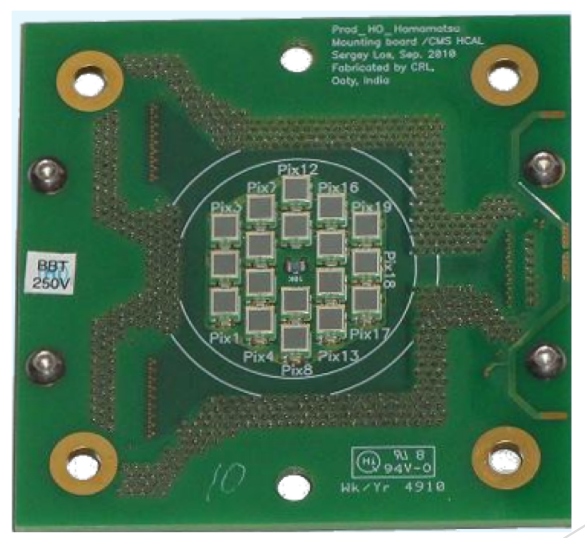
\includegraphics[scale = 0.45]{/home/anter/Desktop/Thesis/Figures/Final/SiPM_2.png}\\
\vspace*{4mm}
\caption[The arrangement of Silicon Photo-Multipliers (SiPMs) on the Mounting Board (MB).]{The arrangement of Silicon Photo-Multipliers (SiPMs) on the Mounting Board (MB). Taken from \cite{DN}}
\label{fig:sipm}
\end{center}
\end{figure} 

\section{Silicon Photo-Multipliers}
A silicon photo-multiplier (SiPM) used in HO is a Hamamatsu Multi-Pixel Photon Counter (MPPC) in a surface mounted device housing. It has a cell pitch of 50 $\micro$m with an active area of 3 $\times$ 3 mm$^2$. The operating voltage required is $\sim$ 70 V with a gain $\sim$ 6 $\times$ 10$^5$ fC/photo-electron when operated at a voltage greater than the breakdown voltage by 1 V. At this over-voltage which is given by the bias voltage subtracted from the breakdown voltage, the typical dark current rate is of the order of a few hundred kHz. Along with the installation of SiPMs, the commissioning of the upgraded parts also took place. The commissioning includes the quick identification of the problems with the new and existing hardware, validation of the installation and repairs, in case of any malfunctions, during the access to the hardware. To monitor and optimize the operational parameters, two types of the data were used : the signals from SiPMs in the absence of light referred as pedestal events (PED) and the charge distributions collected by illuminating the SiPMs with a calibrated light emitting diodes referred as LED events. While performing the Quality Control (QC) analysis, the PED and LED events or runs were taken through an online software created by HO CMS group. These runs were used to study and analyze the properties of SiPMs. 

In the first step of commissioning, a communication test was performed with the readout system along with the verification of slow control operation and channel response. After that, the measurements and optimization of SiPM operational variables were carried out. One of the important quantities of the SiPMs to study is the change of breakdown voltage (BV) and calibration factor gain (G) with the temperature. BV gives the threshold voltage after which the diodes switch to avalanche mode and gain corresponds to the charge produced by SiPM for a single photo-electron (SPE). The gain of SiPMs depends linearly on the temperature with a relative dependence of 8\% gain shift per K at an operating point of 1.5 V over-voltage \cite{Anderson:2011zzc}. As the gain depends linearly on the over-voltage, the change of the breakdown voltage with temperature translates into a change of the gain with temperature. This dependence requires an active control of the temperature of SiPMs with better than 0.1 K stability. So a peltier element is mounted on the back of the MB for cooling purposes in order to stabilize the temperature. We mainly studied the variations of BV and gain with temperature : \\ \newline
{\bf Breakdown Voltage -} The BV can be determined either by using the pedestal spectrum of the SiPMs or the signal of a short LED pulse. In the first method, the gain is estimated by performing a scan of the bias voltage. The dependence of the measured gain on the bias voltage is fitted with a linear function. The extrapolation of fit function to zero gain gives the value of the breakdown voltage. The second method uses the relative change of the measured signal (S) when pulsing an LED and varying the bias voltage (V). The distribution of dS/SdV as a function of V whose maximum provides the BV. This distribution is fitted by a simple Gaussian function to obtain the value of BV. The variation of the breakdown voltage, obtained using the LED method, over time is shown for one RM (18 channels) in Fig.~\ref{fig:BV}. When the detector is operated in stable conditions, it is observed that the BV measurements also stay stable within 50 mV which illustrate the reliability of the BV determination. This variation is studied over a period from the end of January, 2014 to the beginning of March, 2014 which indicates that if any changes are observed in gain or breakdown voltage, they are not caused by changes in the temperature.\\ \newline
\begin{figure}[!h]
\begin{center}
%\vspace*{-10mm}
\hspace*{-5mm}
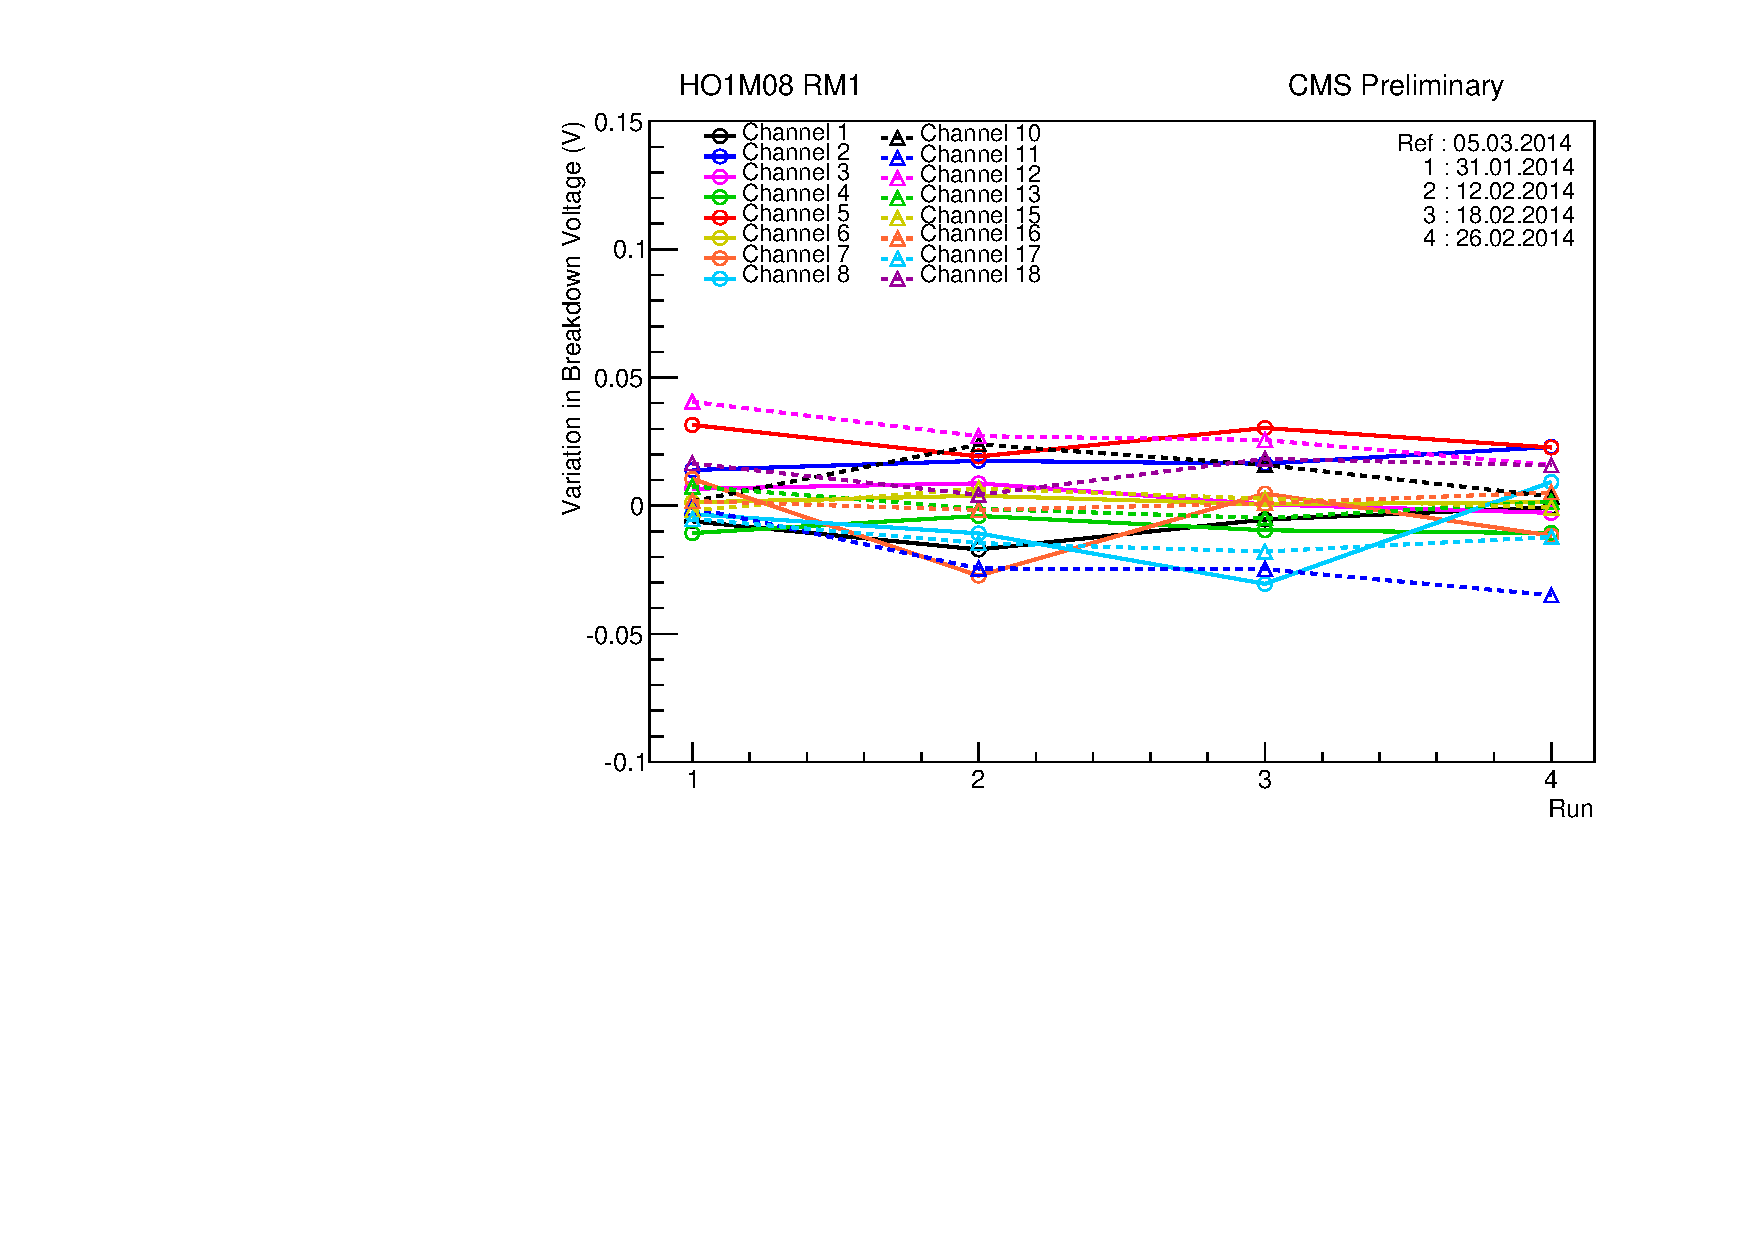
\includegraphics[scale = 0.65]{/home/anter/Desktop/Thesis/Figures/Final/bv_led_iv_49.pdf}\\
\vspace*{4mm}
\caption[The breakdown voltage (BV) is estimated using LED method and its variation is shown over time for 18 channels of one readout module (RM).]{The breakdown voltage (BV) is estimated using LED method and its variation is shown over time for 18 channels of one readout module (RM). When the detector is operated in stable conditions, the BV measurements also are stable within 50 mV illustrating the reliability of the BV determination.}
\label{fig:BV}
\end{center}
\end{figure} \newline
{\bf Gain -} The gain is defined as the factor by which Geiger-mode avalanche (whether initiated by the photoelectric effect or thermal 
carrier excitation) multiplies the initiating electron to form the MPPC’s output charge per avalanche. The gain is determined by generating short light pulses with an LED onto the SiPM. Assuming the intensity of the light pulse not too large and $N$ as number of photons reaching the SiPM, the signal should be equal to $N \times$ gain. According to Poisson statistics, the sigma of the photon number is $\sqrt{N}$ and the sigma of the measured signal is $\sqrt{N} \times$ gain. Dividing the variance of the signal by the mean of the signal one gets sigma$^2$/mean = gain. Figure~\ref{fig:gain1} shows the relative variation of the gain versus time for a single SiPM mounting board. We observed that gain is stable over a time from the middle of February to the beginning of March in 2014 and the relative variation of the gain lies within 2\%. 
\begin{figure}[!h]
\begin{center}
\vspace{-2mm}
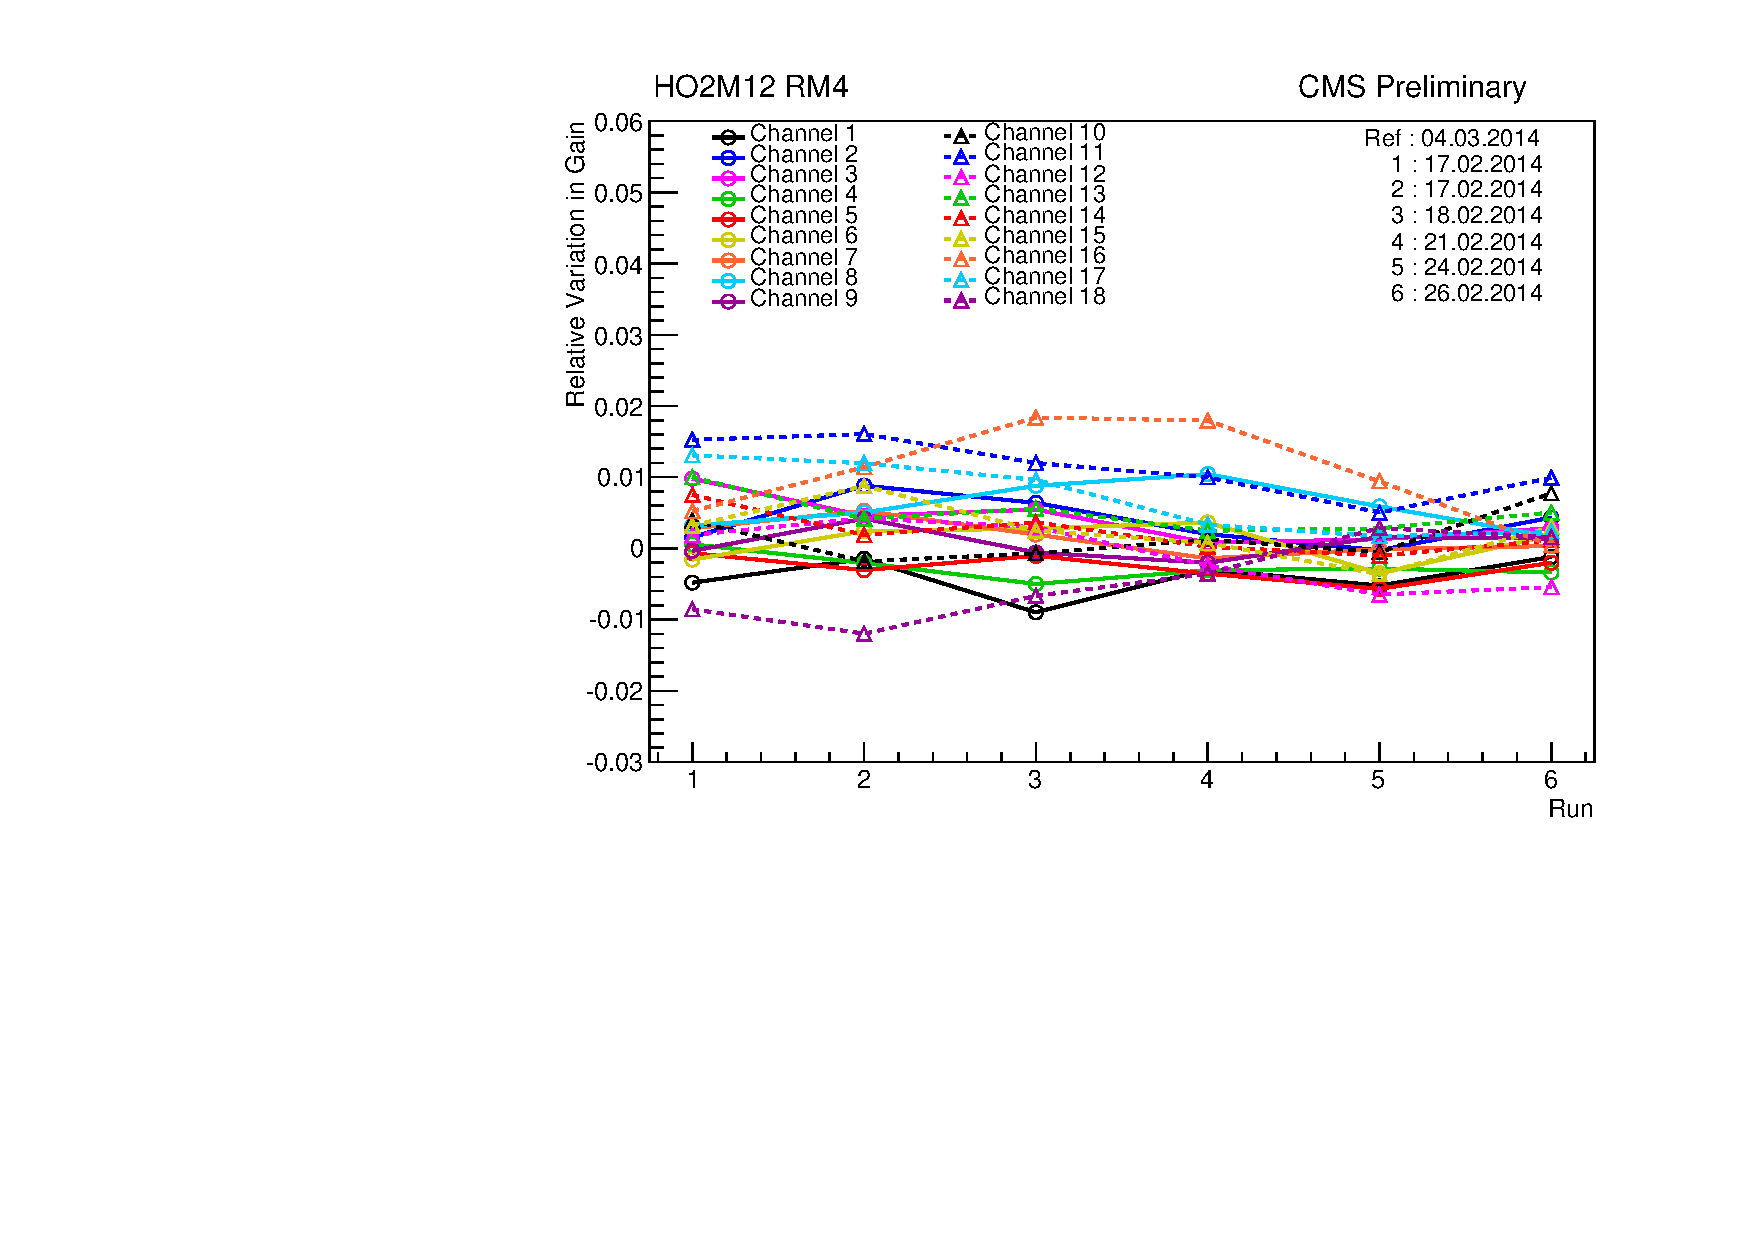
\includegraphics[scale = 0.65]{/home/anter/Desktop/Thesis/Figures/Final/Gain_PED_108.pdf}
\vspace*{4mm}
\caption{The relative variation of the SiPM gain is presented over time for a single RM with 18 channels. The gain is stable over a time from the middle of February to the beginning of March in 2014 and the relative variation of the gain lies within 2\%}
\label{fig:gain1}
\end{center}
\end{figure}\newline
The relative gain variation with time is plotted for all installed SiPMs as presented in Fig.~\ref{fig:gain2} which is fitted using a Gaussian function. The distribution has a width of only 0.5 \% and all gain variations are within 3\%. This illustrates that the gain determination behaves as expected and the operation of the SiPMs with a stable gain is possible. 
\begin{figure}[!h]
\begin{center}
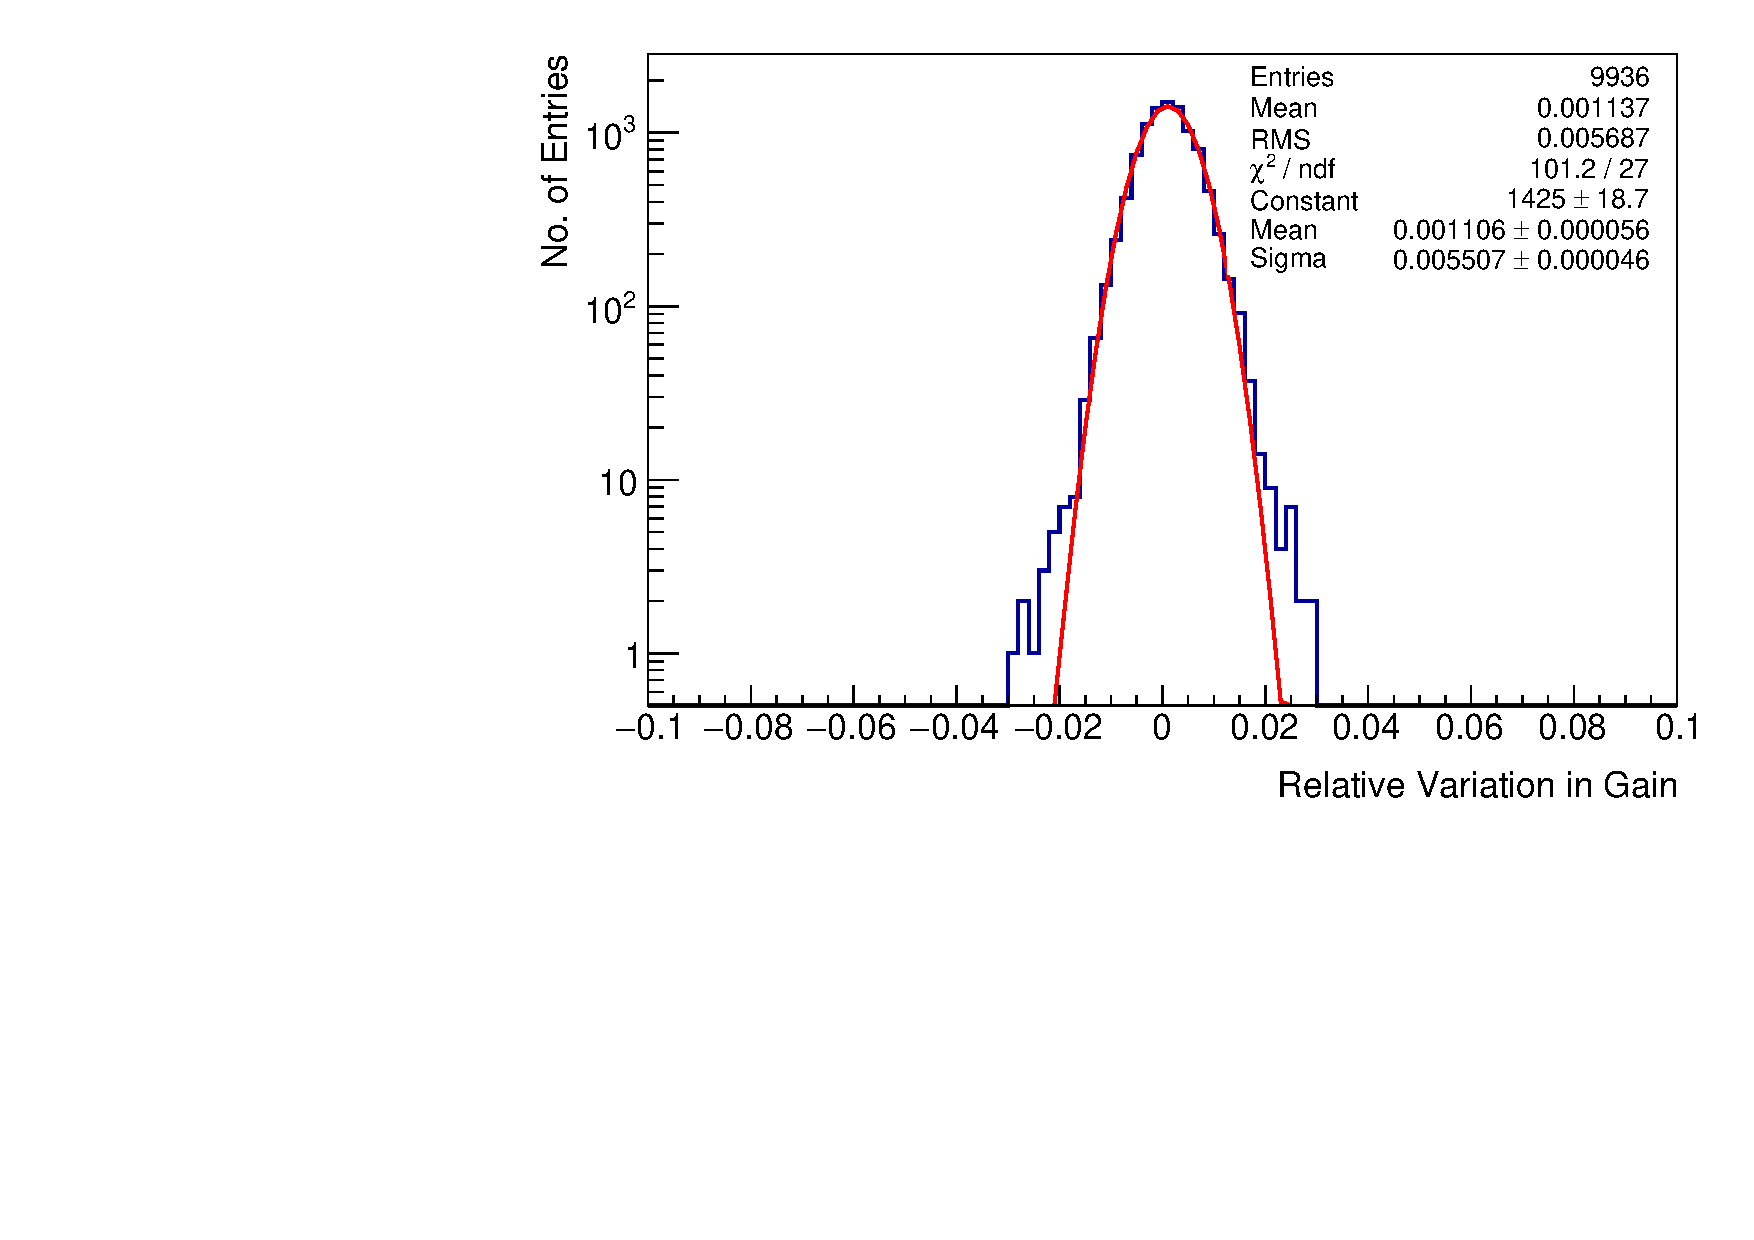
\includegraphics[scale = 0.6]{/home/anter/Desktop/Thesis/Figures/Final/Fit.pdf}
\vspace*{4mm}
\caption{The distribution of the relative variations in gain for all the installed SiPMs is fitted with a Gaussian function. It has a width of only 0.5 \% and all gain variations are within 3\%.}
\label{fig:gain2}
\end{center}
\end{figure}
These results were presented at the CALOR 2014 conference \cite{Kunsken:2015zla} and are documented in Ref. \cite{DN}.

\section{MicroTCA}
During the LHC upgrade at the time of LS1, the increase in LHC luminosity and center-of-mass energy increased the number of interactions per bunch crossing i.e. pileup. Hence, a large amount of the data became available which needed to be processed at a much faster rate than before. This required a very high speed DAQ system and an increase in the number of electronics readout channels to collect high quality data needed to perform physics analysis. Before the upgrade, the VERSAbus Memory card (VME) based system was used but this could not support data transfer rate needed after LS1. So during the upgradation, the existing VME based system was replaced with \mtca (Micro Telecommunications Computing Architecture) standard system in HCAL back-end electronics \cite{CMS:2012tda}. 

The \mtca is an embedded, scalable architecture which offers flexibility to build robust systems. It was designed as a complimentary system to the Advanced Telecommunication Computing Architecture (ATCA), primarily for the core telecommunication networks. It is compact in size and less expensive than ATCA systems.\begin{figure}[!h]
\begin{center}
\vspace*{3mm}
\hspace*{-5mm}
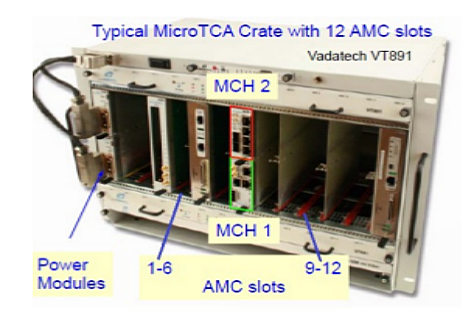
\includegraphics[scale = 0.65]{/home/anter/Desktop/Thesis/Figures/Final/MTCA_2.png}\\
\vspace*{4mm}
\caption[\mtca crate showing the different slots.]{\mtca crate\footnotemark where 12 AMC (Advanced Mezzanine Card) or $\mu$HTR (Micro HCAL Trigger \& Readout) cards can be loaded along with one or two special hub slots occupied by MicroTCA Carrier Hub (MCH) cards. The MCH card is responsible for the control of the power to each slot.}
\label{fig:MTCA}
\end{center}
\end{figure}\footnotetext{Source: \href{https://www.vadatech.com/architecture.php?arcid=2}{https://www.vadatech.com}} \mtca is based on the Advanced Mezzanine Card (AMC) standard which was part of the ATCA. The ATCA standard specifies a crate which can host a large carrier of AMC cards, also known as $\mu$HTR (Micro HCAL Trigger \& Readout) cards. In the simpler \mtca architecture, AMC cards are plugged directly into a backplane such that twelve standard AMC cards can be placed in a crate shown in Fig.~\ref{fig:MTCA}. One or two special hub slots are also present in each crate where at-least one of these slots must be occupied by a MicroTCA Carrier Hub (MCH) card. The MCH card provides the control of the power to each slot and general house-keeping of the crate. The primary MCH site will hold the commercial MCH card responsible for crate management and the ethernet network. The secondary site is used for a CMS-common card, known as AMC13, which is responsible for distributing clock signals to the AMCs. The \mhtr cards receive the data links from the front-ends, calculate and transmit trigger primitives. The Power Mezzanines/Auxiliary Power Mezzanines (PMs/APMs) mounted on \mhtr cards will supply power to them. 

The working of these mezzanines becomes very crucial as their failure may lead to loss of the data collection efficiency. Hence, a Power Mezzanine Testing program was designed to monitor or test \mhtr PMs/APMs for the long term ($\sim$39 hour) stability tests. To carry out these tests, a test-stand was designed as represented in Fig.~\ref{fig:flowchart}. 
\begin{figure}[!h]
\begin{center}
\vspace*{6mm} 
\hspace*{-3mm}
%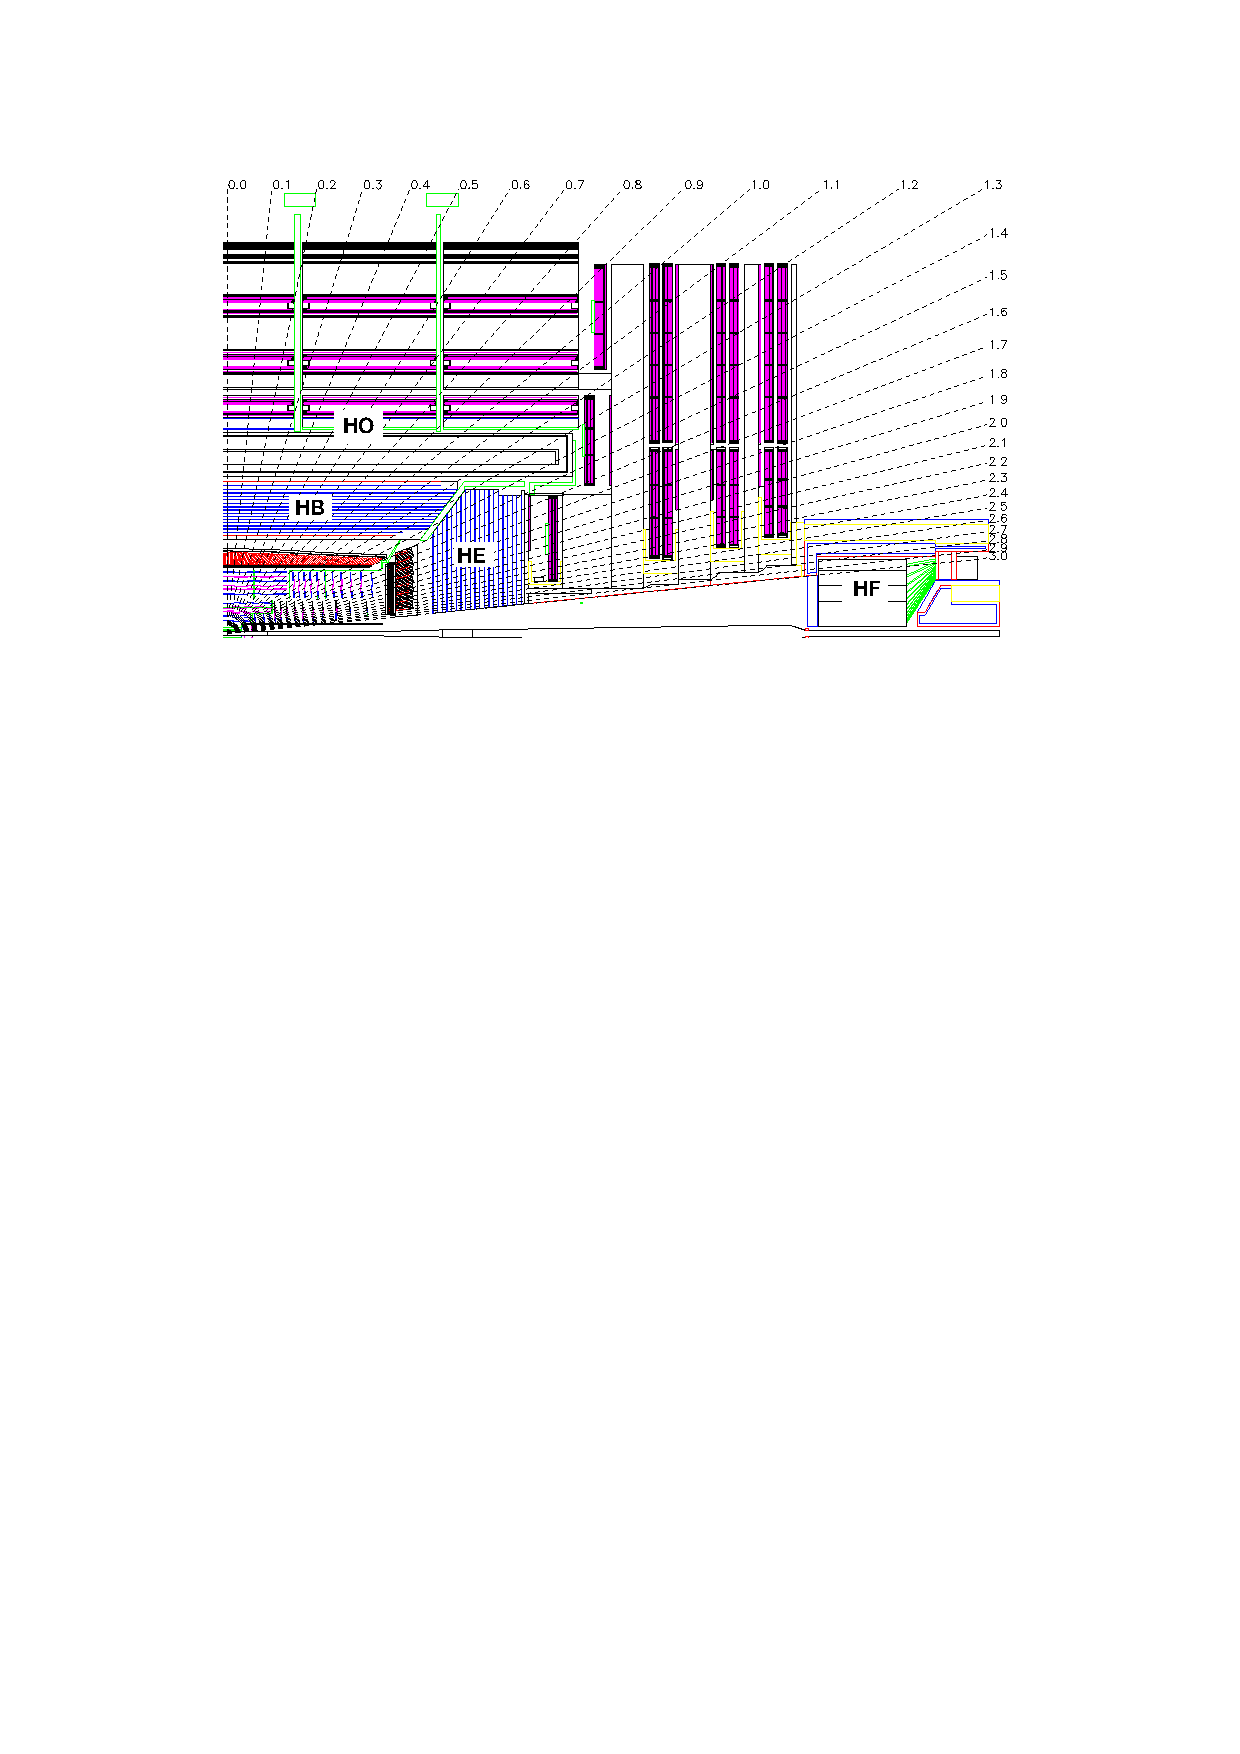
\includegraphics[scale = 1.]{/home/anter/Desktop/Thesis/Figures/edited_cropped_HCAL.pdf}\\
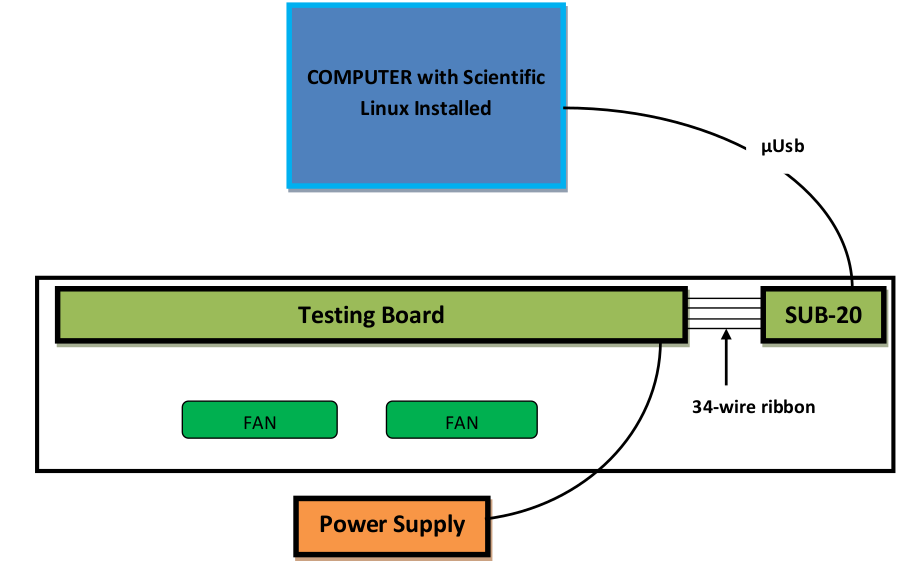
\includegraphics[scale = 0.45]{/home/anter/Desktop/Thesis/Figures/Final/FlowChart.png}\\
\vspace*{4mm}
\caption[A test-stand designed to monitor the working of Power Mezzanines/Auxiliary Power Mezzanines (PMs/APMs) through stability tests.]{A test-stand designed to monitor the working of Power Mezzanines/Auxiliary Power Mezzanines (PMs/APMs) through stability tests. It included a testing board with appropriate slots for mounting PMs/APMs, a SUB-20 module acting as a bridge between testing board and a computer (PC), a 34-pin ribbon wire for a communication between module and PC, a $\mu$USB cable to supply power to module from PC, two fans for cooling of PMs/APMs and a power supply for powering the testing board and PMs/APMs.}
\label{fig:flowchart}
\end{center}
\end{figure} It includes a testing board with 5 slots for mounting 3 PMs and 2 APMs at a time, along with 2 Analog to Digital Converter (ADC) ICs to monitor the temperature, voltage and current. A SUB-20 module acted as a communication bridge between the testing board and a computer (PC) with testing program installed. The SUB-20 module was connected to testing board through I2C (Inter Integrated circuit) and communicated via 34-pin ribbon. A $\mu$USB cable connected the PC and SUB-20 module and also supplied power to module from PC. Two fans were also mounted for cooling of PMs/APMs and resistors embedded into the testing board. A power supply providing voltage of 12 V and current of 10 A was used for powering the testing board and PMs/APMs mounted on it.  

\begin{comment}
\begin{table}[!htbp]
 \centering
 \caption{Four stages of the long term ($\sim$ 39 hour) stability test performed to monitor the working of Power Mezzanines/Auxiliary Power Mezzanines (PMs/APMs).}
 \label{tab:PM_test}
 \vspace{2mm}
 \begin{tabular}{ll}
 \hline\hline
 \centering
 {\bf Test Stages}  & {\bf Duration (Hours)} \rbthm\\\hline
  Marginal Down     & ~~~~~~~~~~~1/2 \rbtrr \\
  Margin Up         & ~~~~~~~~~~~1/2 \rbtrr \\
  Nominal           & ~~~~~~~~~~~19  \rbtrr \\
  High Load Nominal & ~~~~~~~~~~~19  \rbtrr \\
 \hline\hline
 \end{tabular}
\end{table}
\end{comment}

In the Power Mezzanine Testing program, two quick tests namely, Margin Up and Margin Down, were conducted by setting the output voltage 5\% high and low, respectively. Each test was run for a duration of half an hour. These were then followed by long tests with nominal and high load nominal settings, each running for 19 hours. During each test, the output voltage, current, power supplied and temperature of PMs/APMs were monitored and recorded after every 10 seconds. At the end of every test, the average and extremum values of every quantity were used to check the stability of PMs/APMs with time. As a part of the testing of \mhtr cards, we participated in the testing of PMs/APMs for which a test-stand, as shown in Fig.~\ref{fig:mez}, was installed at the Department of Physics, Panjab University, Chandigarh. We successfully tested three sets of PMs/APMs which were then sent to CERN to be used for \mhtr cards. During the CERN visits, we participated in the testing of working of these \mhtr cards at 904 building (Prevessin site in France). The Power Modules required to supply power to \mtca crates were also tested. The tested \mhtr cards were then installed in \mtca crates at CMS P5 site. 

\begin{figure}[!h]
\begin{center}
\vspace*{2mm} 
%\hspace*{-5mm}
%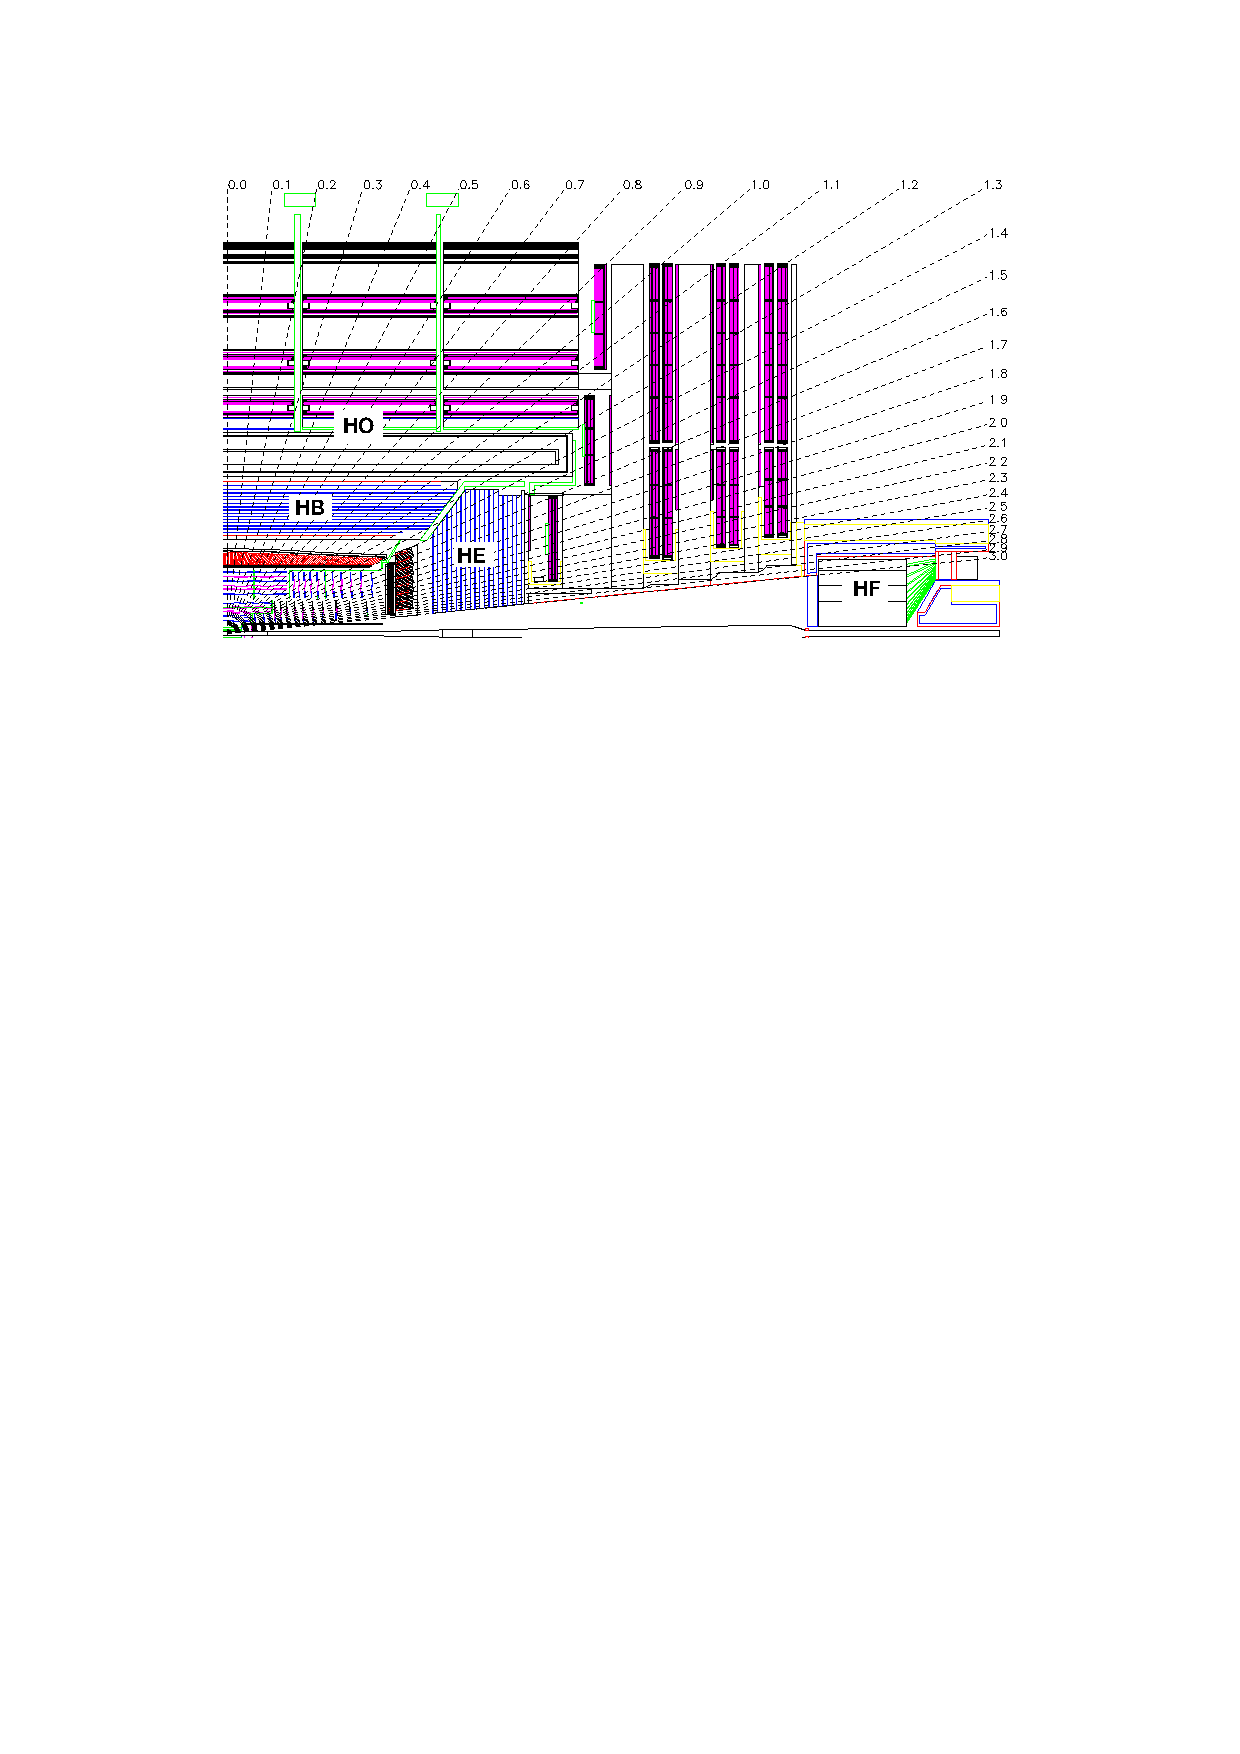
\includegraphics[scale = 1.]{/home/anter/Desktop/Thesis/Figures/edited_cropped_HCAL.pdf}\\
%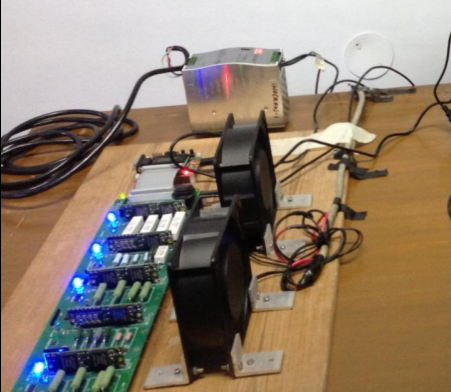
\includegraphics[scale = 0.8]{/home/anter/Desktop/Thesis/Figures/Final/Mezannine_3.png}\\
%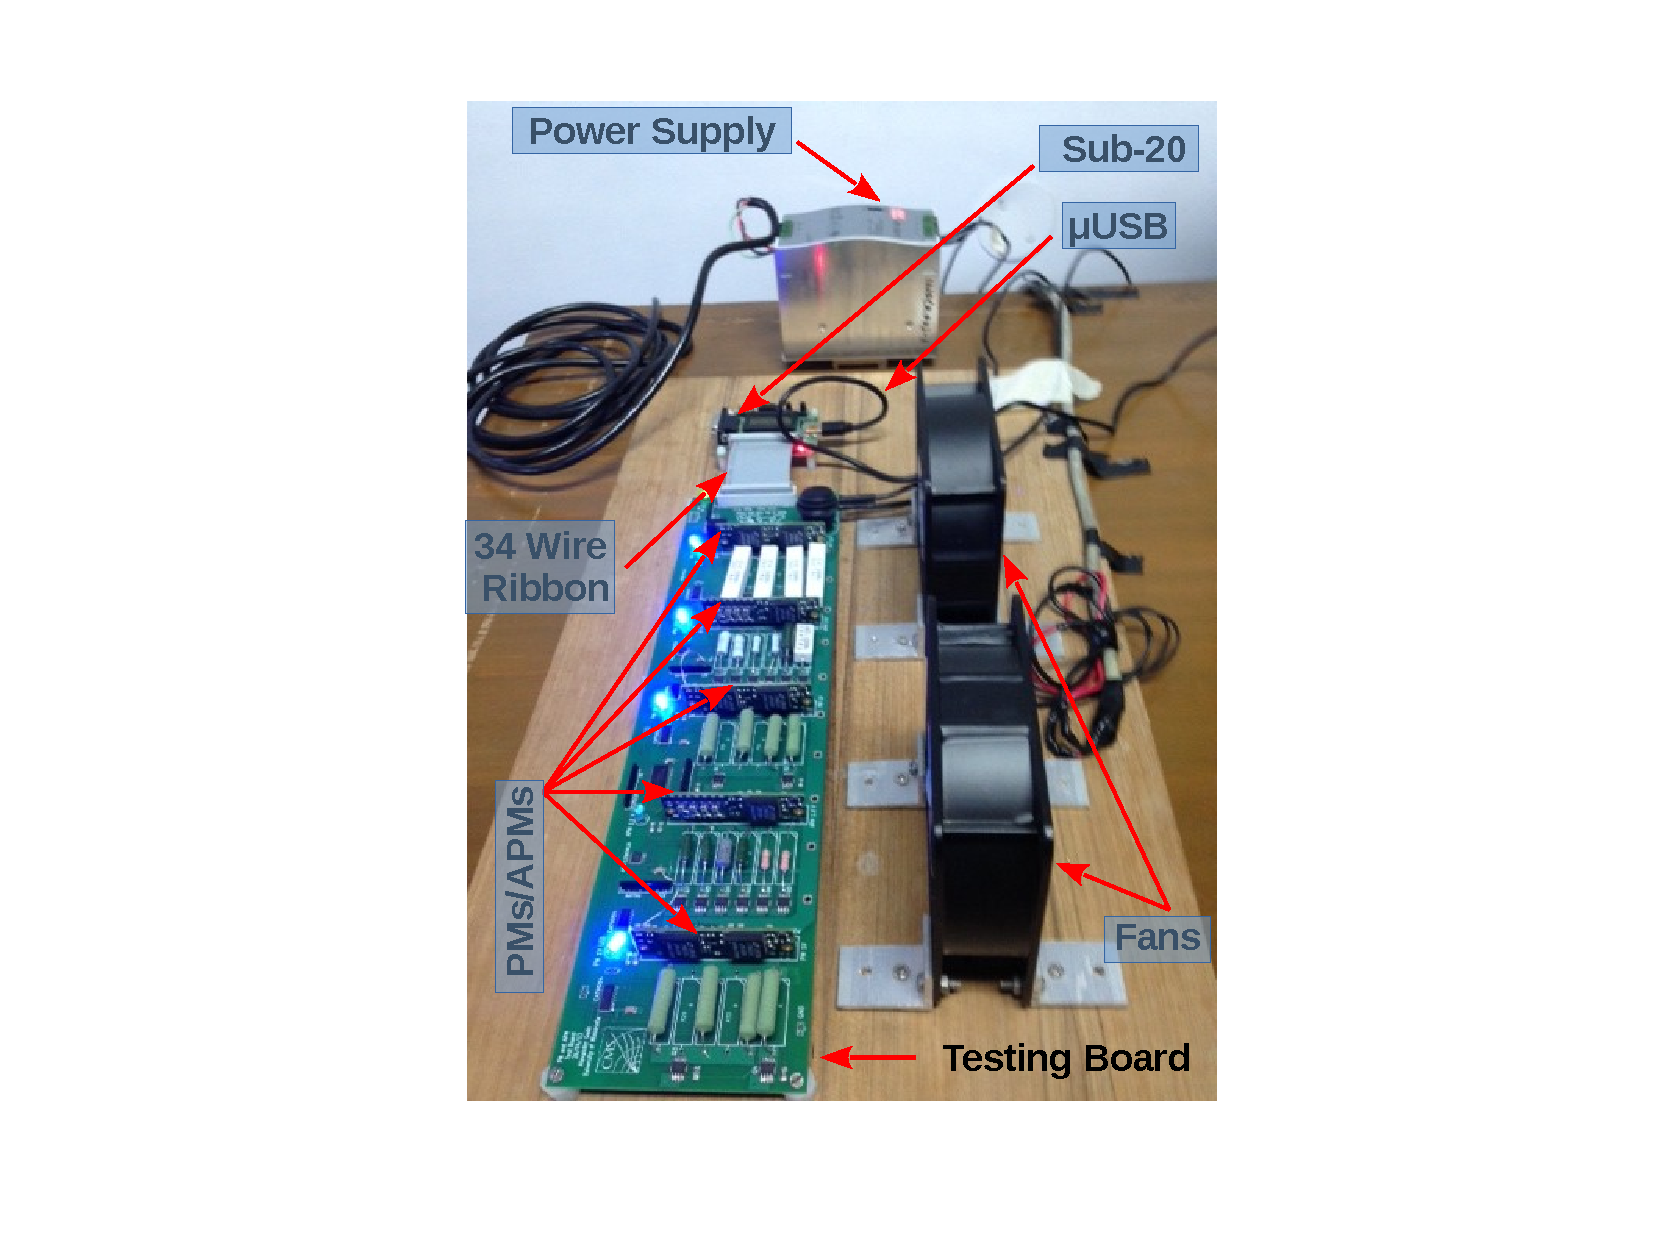
\includegraphics[scale = 0.8]{/home/anter/Desktop/Thesis/Figures/MTCA/SetUp.pdf}
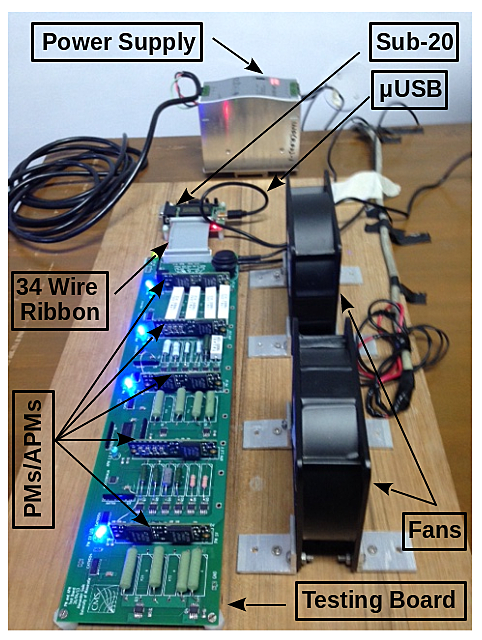
\includegraphics[scale = 0.45]{/home/anter/Desktop/Thesis/Figures/MTCA/SetUp_5.png}
\vspace*{4mm}
\caption{A test-stand installed at Department of Physics, Panjab University, Chandigarh to perform the stability tests for monitoring the working of Power Mezzanines/Auxiliary Power Mezzanines (PMs/APMs).}
\label{fig:mez}
\end{center}
\end{figure}

\section{Other Activities}
Along with performing physics analysis as well as participating in hardware and software activities, I was also involved in service work provided by CMS Collaboration. I worked in the Data Certification (DC) sub-group of the Data Quality Monitoring (DQM) group \cite{DQM} of Physics Performance \& Dataset (PPD) organization for performing the certification of 2016 CMS data. The DQM group is involved in many and major tasks related to CMS data. The DQM organization works at two different levels - online and offline. The online DQM organization takes care of centralization of the various online CMSSW monitoring modules provided by sub-systems and  Detector Performance Groups (DPGs), execution of the live monitoring applications and visualization tool called graphical user interface (DQM GUI) on the DQM cluster and organization of the central online DQM shifts. The online DQM spots problems in the CMS detector while it is running. The offline DQM and DC organization performs centralization of the offline CMSSW monitoring modules provided by DPGs and Data Certification Physics Object Groups (POGs), maintains DQM GUI, used for data certification and release validation and coordinates the certification and publication of the data suitable for physics analysis. I was part of the DC team which was involved in taking the inputs from certification experts, importing their results in CMS Web Based Monitoring's Run Registry (RR) and extracting the information to create the JSON files required for carrying out the physics analysis. In the data certification activity, a list of runs and lumi-sections (LS) is prepared which are good for physics analysis to be performed by the CMS collaboration. For this, one has to :

\begin{itemize}
\item Provide the list of physics runs (cosmics or collisions) to be certified by sub-systems experts
\item Keep the relevant information in the offline RR
\item Provide help to DPG/POG certification experts
\item Update the flags for run data quality depending on the feedback provided by experts
\item Produce the JSON files which includes the final good runs and LS which are then used by physics analysists
\item Announce the official JSON files through physics validation hypernews 
\end{itemize}

More details of the data certification can be found in Ref. \cite{DC}. I also participated in on-going software development of a tool called Historic DQM (HDQM) which is beneficial to study and check stability of various sub-detectors with time.

